\documentclass[11pt,a4paper]{article}
\usepackage[utf8]{inputenc}
\usepackage[spanish]{babel}
%\usepackage{amsmath}
%\usepackage{amsfonts}
%\usepackage{amssymb}
\usepackage{wrapfig}
\usepackage{float}
\usepackage{hyperref}
\usepackage[pdftex]{graphicx}
\usepackage{fancyhdr}
\usepackage[font=small,labelfont=bf]{caption}
\pagestyle{fancy}
\lhead{\bfseries Redes de Datos -- IPv6}
\rhead{}
%\chead{}
\newcommand{\HRule}{\rule{\linewidth}{0.5mm}}
\usepackage[left=2cm,right=2cm,top=2cm,bottom=2cm]{geometry}
\author{Ignacio Perez Laborda -- Barbara Martinez}

\renewcommand{\thefootnote}{\roman{footnote}}

\hypersetup{pdfborder = {0 0 0}}

\begin{document}

\begin{titlepage}

\begin{center}

% Upper part of the page

\includegraphics[width=0.25\textwidth]{./logo_UB.png}\\[1cm] 

\textsc{\LARGE Universidad de Belgrano}\\[1.5cm]

\textsc{\Large Redes De Datos}\\[0.5cm]

%title
\HRule \\[0.4cm]
{ \huge \bfseries Trabajo Practico 2 -- Cloud Computing}\\[0.4cm]
\HRule \\[1.5cm]

% Author and supervisor
\begin{minipage}{0.4\textwidth}
\begin{flushleft} \large
\emph{Alumno:}\\
Ignacio \textsc{P\'erez Laborda}\\
Barbara \textsc{Mart\'inez}\\
\end{flushleft}
\end{minipage}
\begin{minipage}{0.4\textwidth}
\begin{flushright} \large
\emph{Matricula:} \\
502--10426\\
502--10402\\
\end{flushright}
\end{minipage}\\[1.5cm]

\vfill

%Bottom of the page
{\large \today}

\end{center}

\end{titlepage}


\tableofcontents
\newpage
\listoffigures

\newpage

\section{¿Que es IP?}
\subsection{Introducción Histórica}
En plena guerra fría para fines de los años sesenta, el Departamento de Defensa (DoD) norteamericano
necesitaba de un nuevo método para conectar sus distintos centros de investigación y centros 
gubernamentales y que además pueda ser extendida a otros medios de propagación. Esta responsabilidad 
cayo en manos de de ARPA(Advanced Research Projects Agency), la cual en la
reunión de la ACM de 1967 se diseño su estructura básica y se la nombro ARPANET. Para el año 
siguiente se realizaron las primeras adjudicaciones para la implementación de una red de conmutación
de paquetes con una velocidad de 50kbps\footnote{kilobits por segundo}. Dicha implementación fue
adjudicada a la recientemente creada BBN (Bolt Beranek and Newman), la cual fue creada para ese
propósito.\par
Para el año 1969 fue instalado el primer nodo de ARPANET en la Universidad de California en Los
Angeles seguida por los nodos de Stanford, Santa Barbara y la Universidad de Utah. Con estos cuatro
nodos se dio inicio a la red que al cabo de dos años ya se había expandido por todo USA y dos años
después cruzaría el atlántico para desembarcar en Europa.\par
Corriendo el año 1974 ARPANET ya necesitaba de un nuevo protocolo ya que el usado hasta el momento, 
llamado NCP (Network Control Protocol) mostraba muchas falencias al crecer tanto la red. La solución
vino de la mano de un paper que publico Vinton Cerf y Robert Kahn. Este protocolo fue el 
TCP(Transmission Control Protocol), pero este también se enfrento a ciertos problemas y 
restricciones.
\begin{wrapfigure}{r}{0.5\textwidth}
\centering
  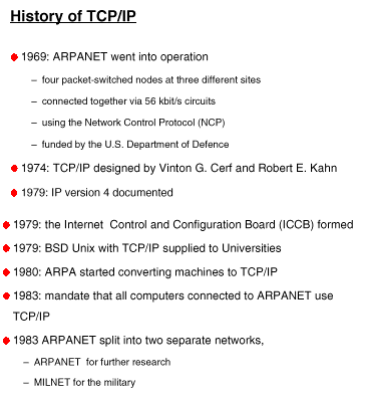
\includegraphics[width=0.48\textwidth]{historiaTCPIP.png}
 \caption[Historia de TCP/IP]{Linea temporal de TCP/IP}
\vspace{-15pt}
\end{wrapfigure}
Para el año 1978 se decidió dividir las responsabilidades entre un par de protocolos; el nuevo IP
(Internet Protocol) que se encargaría de enrutar los paquetes y comunicaciones de dispositivo a 
dispositivo, y TCP para la comunicación confiable de host a host. Aunque son dos protocolos que 
trabajan en capas distintas fueron pensados para operar en conjunto dentro de un conjunto, por eso
comúnmente se los denomina TCP/IP. La version actual, numero 4, del susodicho protocolo y de la cual
hablaremos mas adelante fue especificada en el año 1979.\par
Ya en la siguiente década ARPANET migro completamente a TCP/IP por mandato del Departamento de 
Defensa. En ese mismo año 1983 la red fue divida en dos ARPANET que siguió con su alcance original y
MILNET donde se desempeñarían las comunicaciones militares. Pero otra gran suceso de ese año fue la
inclusión del protocolo en el UNIX de la Universidad de Berkeley, el BSD 4.2.\par
Saltando tres años situándonos en 1986, la National Science Foundation construyo lo que serian los
cimientos de la internet que conocemos al financiar la construcción de una red para la conexión de
sus supercomputadoras. Esto gracias a la apertura de la NSF permitió a particulares conectarse a 
dicha red lo cual ayudo a su gran crecimiento, todo esto estaba y esta apoyado por el TCP/IP. Esta 
red existió hasta el año 1993, para ese entonces se era lo suficientemente maduro y rentable como 
para ser comercial y ya existían empresas dispuestas y con el conocimiento para llevarlo a cabo. Se 
puso en marcha un plan al año siguiente para reducir la influencia de la NFS y aumentar la 
rentabilidad de los incipientes ISP\footnote{Internet Service Provider} privados.\par
Mientras tanto el DoD y el gobierno norteamericano eligieron adoptar el modelo OSI y se pensó que
esto supondría el fin del modelo TCP/IP, incluso el gobierno llego a obligar su uso masivo, pero
TCP/IP siguió evolucionando sobre el fundamento de la practica y su calidad de estándar abierto.\par
Lo que nos puede dejar esta muy resumida historia del protocolo es que la internet no tiene un claro
inventor ni un destino claro, sino fue el trabajo en conjunto de varias personas e instituciones las
cuales querían solucionar sus problemas de comunicación. Fue gracias a las soluciones abiertas las
cuales permitió el mejoramiento por los usuarios, también los niveles de abstracción que se 
permitieron hizo realidad que varias tecnologías puedan convivir en armonía. Esta filosofía abierta
tan característica y que ha marcado tanto a la industria puede resumirse en el lema de la 
IETF\footnote{Internet Engineering Task Force}, expresado por David Clark: "Nosotros rechazamos 
reyes, presidentes y votaciones. Nosotros creemos en el consenso y en el código funcional".

\subsection{El Protocolo IP}
Este protocolo se encuentra en la segunda capa del modelo TCP/IP y la tercera del OSI. El se encarga
de transmitir los paquetes entre el origen y destino basándose en su dirección IP. Esto se logra
encapsulando los datos y formando su propio datagrama. Dentro se tienen dos partes principales el
encabezado y la carga, en el encabezado junto a otra metadata se coloca la dirección IP de origen y 
la de destino. El protocolo IP debe proveer de un servicio no orientado a la conexión no confiable y 
de mejor esfuerzo, también llamado servicio de datagramas. Esto quiere decir: no confiable, el 
protocolo no intenta recuperar los paquetes perdidos; no orientado a la conexión, cada paquete o 
datagrama es manejado independientemente IP desconoce si existe una secuencia lógica de envío; mejor
esfuerzo, IP no garantiza el servicio. Todo esto lleva a que otras capas se encarguen de la perdida
de los paquetes y solicitar su reenvío. IP también permite tres tipos de servicios: Unicast (uno a 
uno), Multicast (uno a varios) y Broadcast (uno a todos).\par
A continuación vemos la estructura de un datagrama de IP.
\begin{figure}[h!]
 \centering
 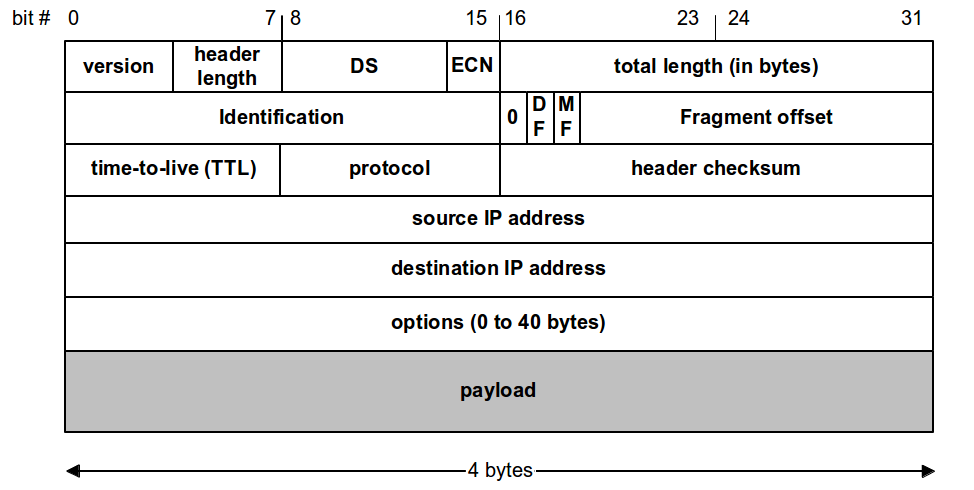
\includegraphics[width=1\textwidth]{ipDatagram.png}
 \caption[Paquete IP]{Paquete IP}
\end{figure}\par
Explicación de los campos:\par
\begin{description}

\item[Version] representa la version del estándar actualmente es cuatro en transición a 6.
\item[Header Length] Tamaño del encabezado en múltiplos de 4 bytes.
\item[DS/ECN] Usado para especificar el nivel del servicio, actualmente no se usa y solo esta
presente para dar compatibilidad retroactiva.
\item[Identification] Identificación única del datagrama de un host, se incremente con cada 
datagrama.
\item[Flags] El primero siempre queda en cero, los otros dos indican si se fragmenta o tiene varios
fragmentos.
\item[TTL] Especifica la cantidad de caminos que puede tomar un paquete hasta que se lo descarte, se
utiliza para prevenir que el paquete quede para siempre dentro de un ciclo.
\item[Protocol] Especifica el numero del protocolo superior.
\item[Header Checksum] El checksum del header.
\item[Options] Restricciones de seguridad, registro de ruta(se agrega la dirección del router por el 
que pasa), marca de tiempo (por cada paso por router) y lista de rutas a pasar (por los únicos que 
puede pasar o por los que debe pasar entre otros)
\item[Padding] Se le agrega para asegurarse que tengo un tamaño de 4 bytes.

\end{description}


\section{El estándar IPv4}
\subsection{Aspectos Técnicos}
Ahora hablaremos de la version 4 del protocolo IP, la cual se implemento para el año 1981 y es 
actualmente el estándar global para internet.\par
El estándar IPv4 utiliza un direccionamiento de 32-bits, lo cual da una posibilidad de tan solo 
4.294.967.296 posibles direcciones, pero de esa problemática nos encargaremos mas adelante. Para 
anotar las direcciones de un método que nosotros los humanos podamos entender se utiliza un sistema 
de 4 octetos expresados en decimal y separados por un punto. Estas direcciones se dividen 
principalmente en dos partes. Una parte la primera es para identificar al ID de la red y la parte
restante identifica al host dentro de la red, ambas juntas como se podrá ver identifican 
unívocamente a un equipo conectado a la red. Históricamente se han dividió las direcciones en clases
dando a una asignación llamada \textbf{direccionamiento con clases}. Se utilizan cinco tipos de 
clases \emph{A, B, C, D, E}
\begin{figure}[h!]
 \centering
 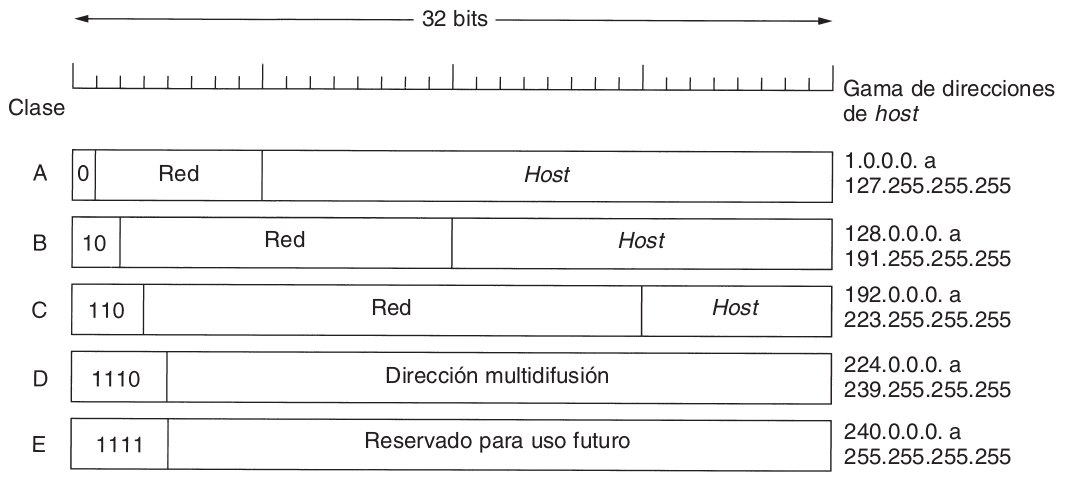
\includegraphics[width=1\textwidth]{clasesIP.png}
 \caption[Clases IP]{Clases IP}
\end{figure}\par
Como se puede apreciar la clase A permite tener muchos hosts por red pero solo puede haber pocas 
redes, por lo cual se utiliza para grandes redes. Además dentro de este rango entran dos direcciones 
reservadas la 0.0.0.0 y la 127.0.0.0 la cual asigna el enlace local, hace referencia a la propia 
interfaz de red, también existe un rango privado dentro de esta red el cual se extiende de 10.0.0.0 
a 10.255.255.255. Esta red puede mantener hasta 16.777.214 de hosts pero solo 128 redes distintas.
La clase B por su parte ya puede ofrecer mas redes por lo que su uso se da para redes de tamaño 
intermedio pudiendo dar cabida a 65.534 hosts pero con un mayor numero de redes posible el cual 
asciende a 16.384 posibles. A su vez el rango de direcciones privada se da entre 172.16.0.0 hasta 
172.31.255.255, también en esta clase se encuentra el link local. Por ultimo tenemos a la clase C la
que menor cantidad de hosts puede soportar, pero si pueden coexistir muchísimas redes distintas 
específicamente 2.097.152 y tan solo 254 hosts en cada red. Por eso esta clase se reserva para redes 
pequeñas. Su rango privado es familiar ya que la gran mayoría de routers hogareños y para pequeñas 
empresas lo utilizan van desde 192.168.0.0 hasta 192.168.255.255. Las dos clases siguientes D y E se
destinan para la multidifusi\'on y para usos futuros respectivamente.\par
Dado que este sistema mostró ciertas falencias para el rápido crecimiento de las conexiones y hosts
necesarios, se desarrollo las subredes y las mascaras de subred. La solución a este problema es 
permitir la división de una red en varias partes para uso interno, pero aún actuar como una sola red 
ante el mundo exterior. Esto se implementa con una mascara la cual tiene una estructura parecida a
la de una dirección IP, un ejemplo seria una mascara donde no existe división la cual quedaría como 
255.255.255.0, solamente el ultimo octeto queda libre para variar seria una mascara para clase C. 
Entonces una mascara de clase A seria 255.0.0.0 y por ultimo una de clase B se expresa 25.255.0.0. 
La mascara permite poder identificar a la subred dentro de la red principal,pero sin que el exterior 
note la división, por lo cual no es necesario solicitar nuevas direcciones. Por Ejemplo, al 
introducirse subredes, se cambian las tablas de enrutamiento, agregando entradas con forma de (esta 
red, subred, 0) y (esta red, esta subred, host). Por lo tanto, un enrutador de la subred k sabe cómo 
llegar a todas las demás subredes y a todos los hosts de la subred k; no tiene que saber los 
detalles sobre los hosts de otras subredes. De hecho, todo lo que se necesita es hacer que cada 
enrutador haga un AND booleano con la máscara de subred de la red para deshacerse del número de host 
y buscar la dirección resultante en sus tablas (tras determinar de qué clase de red se trata). Por 
eso se puede afirmar que la división de redes reduce espacio en la tabla de enrutamiento creando una 
jerarquía de tres niveles, que consiste en red, subred y host.
%\vspace{10cm}

\subsection{Porque Abandonar IPv4}
\subsubsection{Agotamiento de Direcciones IP}
Uno de los mayores problemas que presenta IPv4 es su tamaño, el cual ya ha quedado chico para los
estándares actuales. Este es un numero de solo 32bits con lo cual la cantidad máxima de números
posibles es $2^{32}$ cual da un total de 4.294.967.296 posibles dirección eso es menos de una
dirección por habitante. Esto se ve mas limitante con la llegada masiva de los dispositivos mobiles, 
los cuales se conectan a internet y la entrada de los grandes mercados emergentes del BRIC (Brasil, 
Rusia, India, China).
La introducción de nuevas tecnología, como NAT\footnote{Network Address Translator, traducción de 
direcciones de red},que permiten usar direcciones IP privadas (como al interior de una LAN) para 
comunicarse con Internet a retrasado este inevitable final.\par
Pero quienes se encargan de asignar estas direcciones, esta tarea recae a nivel global en la IANA( 
Internet Assigned Numbers Authority) y 5 RIRs (Regional Internet Registries), los cuales se encargan 
de asignar las direcciones a usuarios finales y registrantes locales tales como los ISP en su área 
designada. Se dividen en:
\begin{figure}[h]
\centering
  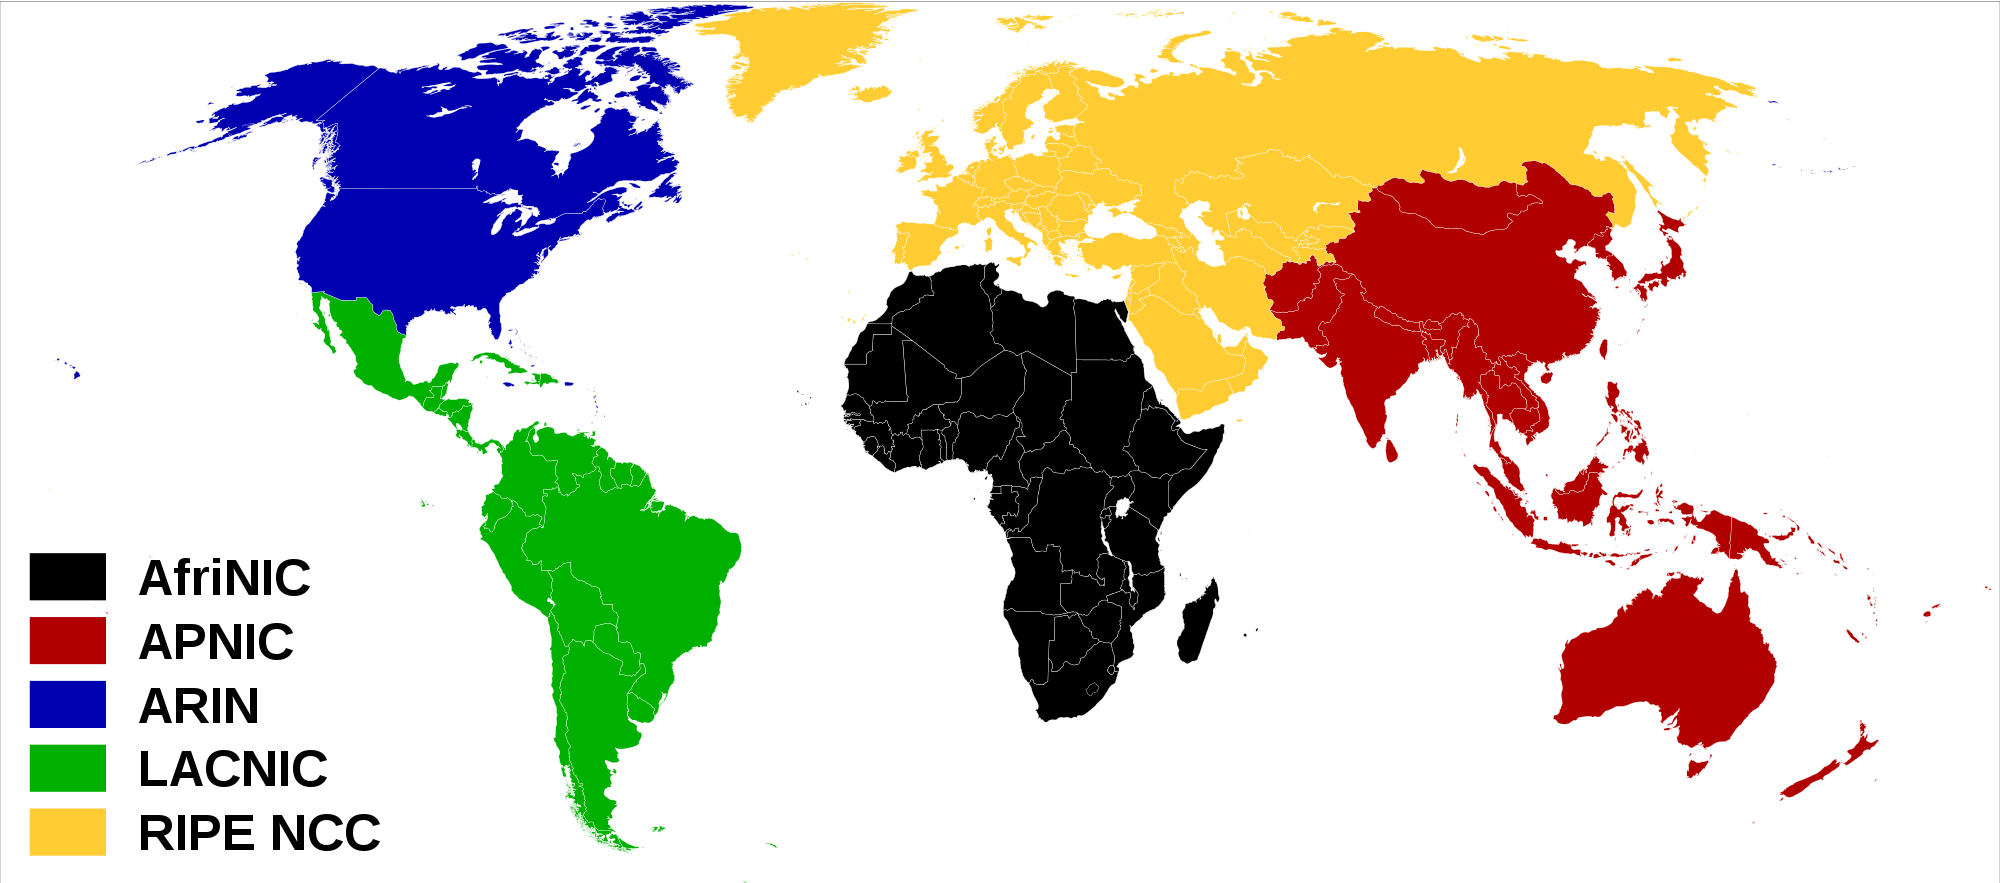
\includegraphics[width=0.67\textwidth]{RIR.png}
 \caption[Las 5 regiones RIR]{Las 5 regiones RIR}
\end{figure}
\begin{itemize}
\item \textbf{AfriNIC} para el continente africano
\item \textbf{APNIC} para la región de Australia, Nueva Zelanda, y asia oriental.
\item \textbf{ARIN} para USA, Canada y partes del caribe.
\item \textbf{LACNIC} para latinoamerica y el resto del caribe.
\item \textbf{RIPE NCC} para europa, Rusia, el medio oriente y asia central.
\end{itemize}\vspace{.2cm}


Ya el 31 de enero de 2011 el IANA agoto su ultimo pool de direcciones libres a esto le siguió el 
agotamiento de APNIC el 15 de abril del 2011 y de RIPE NCC el 14 de septiembre del año 2012, el 
resto se espera que se agote en los próximos años. Esta ya real agotamiento en ciertas regiones deja
de garantizar que se puedan realizar conexiones punto a punto como requieren ciertas aplicaciones
hasta la llegada masiva de IPv6. Para poder controlar la explosión de requerimientos de direcciones.
La APNIC, previo a quedar vacía, restringió a 1024 direcciones a cada miembro.
Para mitigar estos inconvenientes y dado la incompatibilidad entre protocolos, se desarrollaron 
medidas como gateways especiales que interactúan entre ambos.\par
Analizar porque se agotan resulta muy interesante ya que demuestra los cambios sociales y económicos 
de ciertas regiones:
\begin{itemize}
\item Dispositivos Móviles: El alcance masivo de los celulares con capacidad de conexión a internet 
y además las tablets y cada vez mas dispositivos existentes se pueden conectar desde heladeras a 
libros electrónicos, pasando por relojes y autos.
\item Conexiones las 24 horas: Hoy en día es común tener una conexión permanente en las casas y 
dispositivos, la penetración de la banda ancha (que entre otras cosas ofrece dicho servicio) crece 
día a día en todo el mundo. Además como ya se dijo en los celulares y aparatos similares el 3G les 
permite estar también siempre conectados.
\item Demografía: Con el rápido crecimiento económico de países con grandes poblaciones como el BRIC 
hace que se integren millones de personas nuevas a internet, los cuales también tienen mas medios 
para realizar dicha conexión.
\item Uso ineficiente: Dado el repentino crecimiento de internet esta no estaba del todo preparada 
en un principio, cuando fue diseñada nunca se pensó en un uso tan extensivo y al principio se daban 
direcciones de manera indiscriminada y sin mucho control.
\end{itemize}

\subsubsection{Otras Cuestiones}
Además de solucionar el gravísimo problema del bajo numero de direcciones IPv4, este protocolo 
también tiene otros inconvenientes que IPv6 si soluciona de manera mas integrada.
\begin{enumerate}

\item \underline{Simplificación de los encabezados:}\\
La mejora más importante de IPv6 es la simplificación de los encabezados de los datagramas. El 
encabezado del datagrama en IPv6 es más simple que el utilizado en IPv4, así los campos que son 
raramente utilizados han sido movidos a opciones separadas. Aunque las direcciones en IPv6 son 4 
veces más largas, el encabezado IPv6 (sin opciones) es solamente el doble de largo que el encabezado 
IPv4 (sin opciones).

\item  \underline{Seguridad:}\\
Todas las implementaciones de IPv6, en un futuro cercano, deben permitir la opción de utilizar 
IPsec, a diferencia de IPv4 en donde su implementación era opcional (aunque bastante usual), esto 
nos proporcionará más seguridad para el tráfico de paquetes de datos en la red.

\item  \underline{Conexiones más eficaces:}\\
Debido a que se utiliza una cabecera de paquete diferente en IPv6, añadiendo a los datos actuales 
(origen, tamaño, etc.) otros datos tales como etiquetas de contenido, permite optimizar las 
transferencias al poder dar prioridad a tipos determinados de archivos (por ejemplo, dar prioridad a 
los archivos del tipo multimedia o de voz), haciendo a la vez posible que sea el usuario el que 
decida estas prioridades.

\item  \underline{Multicast:}\\
Multicast, la habilidad de enviar un paquete único a destinos múltiples es parte de la 
especificación base de IPv6. Esto es diferente a IPv4, donde es opcional (aunque usualmente 
implementado).

\item  \underline{Autoconfiguración:}\\
Los nodos IPv6 pueden configurarse a sí mismos automáticamente cuando son conectados a una red 
ruteada en IPv6 usando los mensajes de descubrimiento de routers de ICMPv6. La primera vez que son 
conectados a una red, el nodo envía una solicitud usando multicast (router solicitation) pidiendo 
los parámetros de configuración. Si los routers están configurados para esto, responderán este 
requerimiento con un ``anuncio de router" (router advertisement) que contiene los parámetros de 
configuración de la capa de red.

\item  \underline{Desaparición de los NAT:}\\
Muchas organizaciones que no disponen de suficientes números IP deben utilizar direcciones privadas 
que apuntan a un único numero IP o dirección pública, siendo preciso un NAT que dirija el flujo de 
datos desde la red interna a la exterior. Uno de los beneficios de IPv6 será la plena disponibilidad 
de números IP, así se elimina la necesidad del uso de los NAT debido a que hay disponibles 
direcciones IP de sobra, lo que permite que Internet vuelva a ser una red ``entre extremos".
\end{enumerate}

\section{IPv6} 
\subsection{La Llegada de IPv6}
Principalmente internet era un prototipo que se hizo con un protocolo sencillo, nunca se creyó que 
tuviese un crecimiento tan descomunal como para que en el futuro surgieran problemas tales como la 
seguridad entre el tráfico de datos a través de la red, y la implementación de internet en otras 
tecnologías como por ejemplo celulares. Los problemas que hicieron inadecuada la version 4 de IP 
hicieron que se cambiara el sistema por completo por lo tanto los desarrolladores fueron forzados a 
crear un protocolo que resolviera los problemas actuales y trabajara diligentemente para asegurar 
que estos problemas no se encontraran nunca mas. Los desarrolladores del protocolo trabajaron diez 
años pero su implementación se hizo recientemente, es la implementación de un nuevo protocolo, 
escalable, ilimitado y con una gran proyección a futuro.\par

\subsection{Los Beneficios de IPv6}
Entre los principales beneficios de IPv6 fue la solución a dos problemas fundamentales que tenia su 
protocolo antecesor: la falta de direcciones, y la escalabilidad de la ruta. Las soluciones 
implementadas fueron:
\begin{itemize}
\item Incremento de las direcciones IP
\item Desarrollo en la jerarquía de direcciones
\item Organización en los perfiles de red
\item Autoconfiguración sencilla de la red
\item Mejora en la escalabilidad del enrutamiento
\item Enrutamiento a la mejor dirección posible(Anycast)
\item Mejoras en la seguridad
\item Mejoras en la movilidad
\item Se agregan nuevas tecnologías que mejoran la performance del protocolo
\end{itemize}

\begin{figure}[h!]
 \centering
 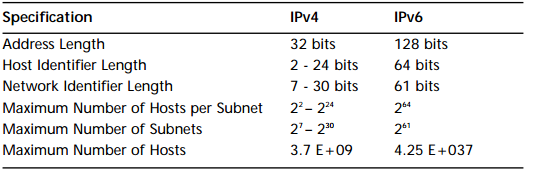
\includegraphics[width=0.8\textwidth]{comparativo_ip.png}
\caption[Comparación versiones IP]{Cuadro comparativo de las direcciones IP}
\end{figure} \par

\subsubsection{Jerarquía de Direcciones}
IPv6 divide las direcciones en distintos ámbitos definidos o limites en los cuales se delegan las 
direcciones, por lo que soluciona problemas de disgregación. Cuenta con un sistema de enrutamiento 
que permite discernir rápidamente el tipo de paquete que es, así el enrutamiento se realiza de una 
forma mas sencilla y eficiente.
Otra de las herramientas que cabe destacar en IPv6 es el agregador de nivel superior \textbf{Top 
Level Aggregator (TLA)} que consta de dos propósitos: el primero es la designación de un gran bloque 
de direcciones compuesto por pequeños bloques que tienen la función de dar una conectividad 
descendiente a los que necesitan acceso a la red. El segundo es la detección de la ruta de origen, 
resulta mas claro ver quienes son los que tienen bloques de direcciones de proveedores y quienes son 
los que tienen una dirección local. Esto aumenta la eficiencia del núcleo de internet porque al 
agruparse de esta forma y haber una mejor organización de las direcciones, es mucho mas claro el 
pasaje de información.\par
Otro de los organismos existentes en este protocolo es el \textbf{NLA Next Level Aggregator} que si 
bien es demasiado pequeño para ser clasificado como un TDA, tiene una cadena principal regional 
extensa y cuenta con un numero de pequeños clientes. Sirve para dentro del gran bloque que 
proporciona el TDA, romper su porción de direcciones y delegar las direcciones obtenidas a los 
\textbf{Sitios Agregadores de Servicio SLA}. Estos SLA se encargan de identificar subnets que no 
estén en el sitio.Otro beneficio importante que se puede destacar del NLA se relaciona con la 
estabilidad de ruta actual de todas las rutas a nivel mundial dejando de lado las inestabilidades 
conocidas como cortes, fallo en enlaces y lentitud en el tráfico de datos. Debido a esta 
inestabilidad, el concepto de ``route dampening" surgió y trabaja de la siguiente forma: cada vez que 
una ruta se retira y se renuncia, se le asigna una penalización que se mantiene hasta el lugar donde 
se encuentra la inestabilidad que por lo general suele ser una frontera exterior o  protocolo de 
puerta de enlace. Mientras mas alta sea la inestabilidad, mas alta será la penalidad asociada con la 
ruta. Cuando esa penalización alcanza cierto nivel, la ruta se retira y debe someterse a un período 
de espera. Mientras mas tiempo pasa, la pena va decreciendo hasta que la misma se disuelve y vuelve 
a estar permitida y se la reinserta en la tabla  de BGP del router. El propósito de esto es proveer 
una forma de negociar las inestabilidades de una forma tal que se minimice el costo de otros 
procesos que son importantes.\par
Cabe destacar que otro beneficio importante de la agregación la mejora importante en el 
enrutamiento, que forma parte de un requisito fundamental en IPv6. Así como hay mas direcciones 
también hay extensas ramificaciones y formas de organizarlas y controlarlas para que la asignación 
de las mismas  no sea un problema.

\subsubsection{Un Mecanismo de Direccionamiento  mas Sencillo}
El modelo IPv6 esta  caracterizado por tener una dirección de 128. Los primeros 64 bits están 
destinados a la numeración de red y los últimos 64 se utilizan para la numeración del host, al tener 
128 bits es mucho mas variada la cantidad de direcciones que se pueden formar y también aumenta la 
seguridad de la red. Debemos recordar que los últimos 64 bits del id del host se obtienen a partir 
de las direcciones MAC de la red de interfaz. Por convención la primera dirección se da normalmente 
al enrutador designado y el resto de las direcciones se asignan a los host de la subred con el 
ultimo domicilio. En IPv6 es un tanto diferente ya que  sabemos que la id es una dirección  de 64 
bits que se obtiene de la dirección MAC. Hoy en día las direcciones MAC son de 48 bits, para llegar 
a 64 bits se las rellena con cadenas cadenas 0xff y 0xFE (: FF: FE: en términos IPv6) para cubrir la 
diferencia que existe entre la dirección MAC de la identificación de la compañía y el ID 
proporcionado por el proveedor de la MAC.\par
El conflicto reside en si es necesario que las direcciones MAC tengan que cambiar su longitud  solo 
porque con el protocolo IPv6 cambia las longitudes del direccionamiento, si la necesidad de 
implementar direcciones MAC tan largas, la siguiente opción para la longitud proporcionara mas de 
$1.8 \times 10^{19}$ direcciones MAC en lugar de usar (264-248) si este viene a ser el
caso, simplemente puede dejar el relleno de la dirección MAC, y el uso de los 64 completo
bits de la dirección MAC para el ID de host.

\subsubsection{Autoconfiguración de Direcciones}
La mejor ventaja de IPv6 sin dudas es la capacidad de autoconfiguración de las direcciones IP. Antes 
de entrar en detalles sobre el tema hablaremos de \textbf{la dirección de multidifusión}. Esta 
consiste en una dirección multicast que se puede asignar simultáneamente a mas de una maquina.Esta 
dirección envía los paquetes al grupo de equipos asignados a la misma.Todas las maquinas que están 
asignadas a esa dirección se dice que están en un grupo multicast, cuya dirección es la dirección  
de multidifusión que utilizan.Los equipos conectados envían y reciben datos desde mas de un host. Se 
utiliza este estilo para realizar 1 a N o M transacciones.\par
Asociando este concepto con el de autoconfiguración, se puede decir que una red lan es un grupo de 
maquinas y que cuando una nueva maquina ingresa a ese grupo, esta conectada y usan IPv6, se le 
enviara a esa maquina nueva un paquete de multidifusión, este paquete se destinara a la dirección 
de un ámbito local. Cuando el router ve que este paquete entra, este se puede responder con la 
dirección de red de la maquina nueva. La respuesta recibe el paquete y a su vez, lee el numero de 
red que el router tiene enviado. Si se asigna una dirección de IPv6 añadiendo su ID de host. Todo 
este proceso no requiere ninguna intervención manual por parte del administrador, esto asegura 
también la unicidad de la dirección, la maquina esta garantizada para tener la dirección única, 
porque el numero de red exclusivamente asignado por el numero de router de esa red.
Este mecanismo ahorra al usuario un montón de problemas tales como la configuración manual cuando el 
equipo se mueve de una red a otra, la realización de un seguimiento de las direcciones que se ha 
asignado y cuales están libres en un tiempo dado.
Esto le da una facilidad muy grande al administrador de redes ya que no debe perder tiempo en tareas 
de seguimiento y en el renombramiento de la red.

\subsubsection{Mejora en la Escalabilidad del Enrutamiento Multicast}
En este apartado ampliaremos mas el concepto de dirección de multidifusión: En los inicios de 
internet, los problemas de congestión fueron tolerados ya que los datos que enviaban y recibían los 
usuarios no tenían porque ser en tiempo real. Hoy, por el contrario, las empresas están utilizando 
internet para una amplia gama de aplicaciones. Esta tendencia de tener en nuestros dispositivos de 
información tal como el estado del tiempo, la cotización de la bolsa y las noticias del día entre 
otros, hace que se provoque la necesidad de un nuevo tipo de envío de trafico en el cual se pueda 
enviar un conjunto de datos a muchas personas. Antiguamente se copiaba el archivo a enviar tantas 
veces como destinatarios existían y se los enviaba a cada uno. El problema con este método es cuando 
se quiere difundir un archivo en tiempo real de forma masiva, el ancho de banda quizás no sea lo 
suficientemente grande como para manejar tal velocidad de datos. La idea de la multidifusión 
justamente es tomar ese conjunto de datos y enviarlo por una dirección de multidifusión, un grupo 
colectivo de direcciones por ejemplo en IPv4 se utiliza el intervalo de 224.0.0.0 a 239.255.255.255. 
Cuando se quiere enviar algo a múltiples destinatarios, se asigna una dirección temporal del 
intervalo para escuchar los paquetes que llegan del origen. Este concepto nos ayuda a ahorrar mucho 
ancho de banda y velocidad de datos además de mantener una estructura de enrutamiento eficaz \par
En IPv6 es posible asignar ciertas secuencias de multidifusión para ser transferido dentro de un 
área determinada y no permitir que los paquetes salgan de esa zona, los limites de envío y recepción 
de paquetes serán bien conocidos y entendidos por todos.

\begin{figure}[h!]
 \centering
 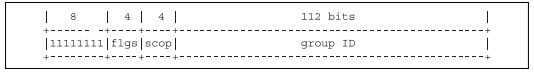
\includegraphics[width=0.7\textwidth]{formato_multicast.png}
 \caption[Formato Multicast]{Formato de una dirección multicast en IPv6}
\end{figure} \par
En la figura de arriba podemos ver el Formato de una dirección multicast. Todos los ocho bits se 
establecen en uno, lo que permitirá a un dispositivo de enrutamiento saber inmediatamente si el 
paquete es de multidifusion y sujeto a la manipulación asociado con su tipo. Los siguientes cuatro 
bits se utilizan para los "flags": los tres primeros flags son reservados y no están definidos por 
lo que están establecidos en cero, el cuarto bit se lo conoce como bit T y se utiliza para decidir 
si la dirección multicast es una dirección permanente o una asignación temporal como se ha hablado 
en el párrafo anterior. Ese ultimo campo nos informara si la dirección de multidifusión que se esta 
utilizando es la que viene de serie. El siguiente campo nos dirá hasta que punto puede llegar la 
multidifusión, en lo que áreas de un dominio de enrutamiento de un paquete puede viajar y la 
dirección del grupo que puede ser alcanzado. Toma los siguientes valores:\par

\begin{figure}[h!]
 \centering
 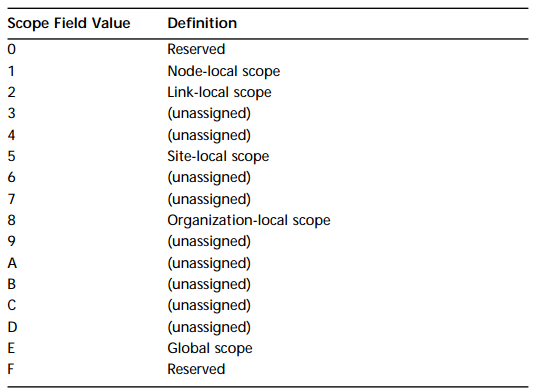
\includegraphics[width=0.71\textwidth]{valoresM.png}
 \caption[Valores del campo scope]{Valores que puede tomar el campo ``scope"}
\end{figure} \par

Dependiendo de como asignemos nuestra dirección multicast, podremos controlar que tan lejos viajarán 
los paquetes. Ejemplo; no es lo mismo la difusión masiva de un vídeo a una cantidad muy grande de 
usuarios que la difusión de un ppt a un grupo de trabajo que se encuentra dentro de la misma red 
LAN. Esto significa que se controlará la propagación de información y que información será propagada 
y a quien se la enviará, por lo tanto, en lugar de dejarle a un administrador de red la tarea de 
colocar filtros para que algunos paquetes le lleguen a cierta gente y a otros no, podemos dejarle 
esta tarea a este mecanismo. Esto también permite una fácil configuración de un nivel de privacidad 
y muy bien definido, que también facilita el mantenimiento del mismo.

\subsubsection{Dirección Anycast}
IPv6 implementará un nuevo tipo de dirección, la dirección \textbf{anycast}. Este tipo de dirección 
mejora la eficiencia del enrutamiento, pero antes de explicar cómo lo hace, pasaremos a definir de 
qué se trata este nuevo tipo de dirección:
Esta dirección de IPv6  esta asignada a un grupo de uno o mas hosts que tienen un propósito en 
común. Cuando los paquetes son enviados a la dirección anycast, la dirección decide a qué equipo del 
grupo va a enrutar primero el paquete analizando cual es el mas cercano a la fuente del mismo que se 
determina por la \textbf{IGP}\footnote{Interior Gateway Protocol} de la red en cuestión.Esto 
dispersa la funcionalidad geográficamente por lo tanto aporta una notable diferencia en dos 
sentidos. Si bien el formato multicast y el anycast son para mas de una maquina host, la dirección 
anycast sirve para la transmisión de datos uno a uno mientras que la multicast sirve para uno a 
muchos.\par 
Este tipo de dirección ahorra mucho tiempo al usuario en la recepción de paquetes ya que el equipo 
mas cercano al equipo fuente será el que le tome menos tiempo en llegarle la información y así 
sucesivamente, además de ahorrar ancho de banda ya que la distancia entre un paquete  es minimizada, 
y al usar menos ancho de banda también se ahorra dinero. En una dirección de formato anycast las 
maquinas están enumeradas.
\begin{figure}[h!]
 \centering
 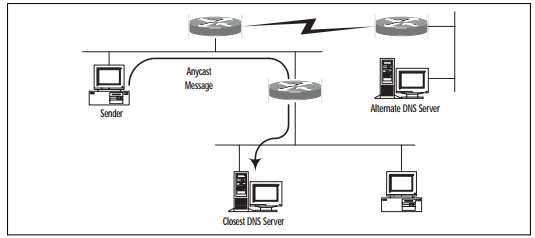
\includegraphics[width=0.71\textwidth]{anycast.png}
 \caption[Esquema anycast]{Esquema de cómo trabajan las direcciones anycast}
\end{figure} \par

\subsubsection{La Nueva Cabecera del IPv6}
La nueva cabecera que implementará el IPv6 solo tiene seis campos y dos direcciones que a diferencia 
del IPv4 que contiene diez campos arreglados, dos direcciones y un campo opciones de tamaño 
variable.
\begin{figure}[h!]
 \centering
 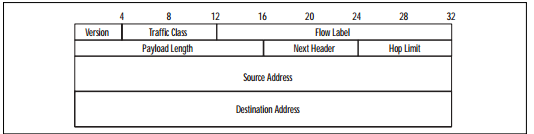
\includegraphics[width=0.71\textwidth]{ipv6head.png}
 \caption[Valores del campo scope]{Esquema que muestra como es la cabecera de IPv6}
\end{figure} \par
Las cualidades importantes que resaltan la sencillez de esta nueva cabecera son:
\begin{description}
\item[Formato Simplificado] Se simplifico la cantidad de campos de la cabecera,también se quito la 
variable de tamaño opcional. Este formato simplificado aporta mayor flexibilidad al protocolo.
\item[No hay checksum de la cabecera] fue eliminado el checksum de la cabecera, este campo fue 
incluido en IPv4 porque  se necesitaba asegurar la integridad de los datos. Ahora, al ser Internet 
mucho más veloz no se necesita esta herramienta, además de que ahora el checksum se realiza en el 
host, no en el router.
\item[Salteo de fragmentación del Procedure] En IPv4 , los router fragmentaban paquetes que eran 
demasiado largos para la transmisión directa. Esto significaba un esfuerzo extra que consistía en 
fragmentarlos para su transmisión. En IPv6 solo el host puede fragmentar el paquete. Para ayudar al 
host, IPv6 incluye una función que encuentra la máxima unidad de transmisión(\textbf{MTU}) tamaño 
del origen hacia la transmisión.

\end {description}
\begin{figure}[h!]
 \centering
 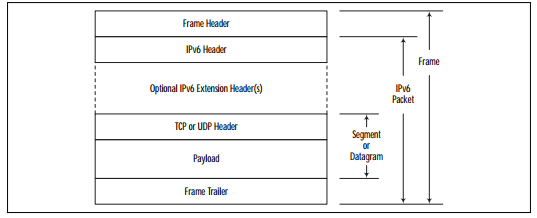
\includegraphics[width=0.71\textwidth]{header.png}
 \caption[Cabeceras IPv6]{Esquema que muestra como es la cabecera de IPv6}
\end{figure} \par
\subsubsection{Seguridad}
IPv6 es mas seguro porque puede soportar seguridad basada en encriptación interoperable. IPv6 
integra seguridad a su arquitectura introduciendo dos extensiones de cabecera opcionales: La 
cabecera de autenticación y la cabecera \textbf{ESP}\footnote{Encripted Security Payload}. Pasaremos 
a describir brevemente cada una. 
\begin{description}
\item[Cabecera de Autenticación] su secreto es un valor que chequea la integridad de los campos 
(\textbf{ICV}\footnote{integrity check value}), este es computado por el origen y nuevamente 
computado por el destino.
\item[Salteo de fragmentación del Procedure] En IPv4, los router fragmentaban paquetes que eran 
demasiado largos para la transmisión directa.Esto significaba un esfuerzo extra que consistía en 
fragmentarlos para su transmisión. En IPv6 solo el host puede fragmentar el paquete. Para ayudar al 
host, IPv6 incluye una función que encuentra la máxima unidad de transmisión(\textbf{MTU}) tamaño 
del origen hacia la transmisión. Proporciona integridad entre ambos puntos y autenticacíon de los 
datos de origen, también verifica la integridad del origen de los datos, contiene un campo llamado  
numero de secuencia que se utiliza para detectar los replays de los paquetes. También con esta 
cabecera se puede detectar la llegada de un paquete con IP duplicada.
\item[Cabecera ESP] Contiene un parámetro de índice de seguridad (\textbf{SPI}) que refiere a una 
asociación de seguridad informándole al destinatario como esta encriptada la utilidad. Cuando se 
crea un túnel, esta  cabecera original se encripta junto con la utilidad y se manda por un IPv6 
externo y una cabecera ESP externa también. Una puerta de enlace separa la información y la 
decodifica.Esto hace que el tráfico no se atasque.
\end {description}
\subsubsection{Movilidad}

Cuatro conceptos fundamentales acerca de la movilidad:
\begin{itemize}
\item Direccion Hogareña
\item Dirección de Atención
\item Encuadernacíon
\item Agente hogareño

\end {itemize}
las IPv6 móviles son identificadas por un una dirección hogareña, sin importar a cual estén 
asociadas al momento. Cuando un host móvil cambia a uno de una subred a otra, se necesita una 
dirección de atención para llevar a cabo el proceso de autoconfiguración dentro de la subred. La 
asociación entre la dirección hogareña y la dirección de atención se llama encuadernamiento. Cuando 
el dispositivo adquiere su dirección de de atención le notifica al agente hogareño de este cambio de 
estado con un mensaje de  actualización de encuadernamiento, el agente mantiene lo que se llama un 
cache de encuadernamiento que es el mapeo entre ambas direcciones la de atención con la hogareña.
\par Un host movil se puede alcanzar mediante el envío de un paquete a su dirección hogareña o local 
también podríamos llamarla.Si esta dirección esta conectada a la red domestica, e l agente de origen 
reenviará el paquete al host móvil a través de su dirección de atención.Entonces enviara un mensaje 
de actualización al nodo de origen, se actualizará y enviará los paquetes subsiguientes directamente 
al nodo móvil a través de su atención  de la dirección. \par 
Los propósitos de esto básicamente son orientados a los teléfonos celulares.
\subsubsection{Performance/Rendimiento}
IPv6 incluye mejoras en el rendimiento y la escalabilidad.

\begin{description}
\item[Reducción de la traducción de direcciones] En IPv6 la traducción de direcciones para superar 
las limitaciones de espacio no es necesaria, a diferencia de IPv4 que solo utiliza direcciones 
privadas limitadas dentro de la red privada.
\item[Reducción de gastos de enrutamiento] las direcciones IPv6 asigna a través de servicios 
proveedores para fomentar una jerarquía de direccionamiento que reduce el enrutamiento exagerado.
\item[Ruta mas estable en IPv4]Resultados de una ruta cuando un enlace fiable es repetidamente 
retirado y volver a ser advertido, el procesamiento de estos cambios de enrutamiento supone una 
carga para Internet. En IPv6, un solo proveedor puede agregar las rutas de muchas redes y permiten 
aislar la red del proveedor.
\item[Reducción de difusión] IPv6  utiliza el descubrimiento de vecinos para realizar una función 
similar durante el proceso de configuración automática sin el uso de difusiones ARP
\item[Multicast con ámbitos de enlace] IPv6 contiene una dirección de multidifusión que contiene un 
campo de alcance que puede restringir los paquetes de multidifusión para el nodo, el enlace o la 
organización.
\item [Cabecera Simplificada] IPv6 Posee un encabezado aerodinámico de ocho campos de longitud 
fija. Estas cabeceras reducen la sobrecarga de la red.
\item[No Fragmentación del nodo intermediario]IPv6 proporciona el MTU Discovery que es una función 
para determinar el tamaño del MTU y para el camino desde el origen hacia el destino
\item[No existencia del checksum de cabecera]IPv6 no necesita ese checksum de cabecera ya que la 
fiabilidad de los enlaces de red de hoy en día reduce la probabilidad de que los paquetes sean 
erróneos.Reduce la carga de la red.
\end{description}

\subsection{IPv6 vs IPv4}
\subsubsection{Estructura de Dirección}
IPv6 cuenta con una dirección de 128 bits de longitud y comprendido por un prefijo de subred y una 
interfaz de identificación.En ambos protocolos el prefijo y la cuentan con 64 bits de largo, pero el 
prefijo de subred es el numero de red asignado al vinculo, el identificador de interfaz deriva de la 
dirección MAC. Durante la configuración de la red IPv6 el nodo host remplaza su propia ID de 
interfaz por una ROM.

\begin{figure}[h!]
 \centering
 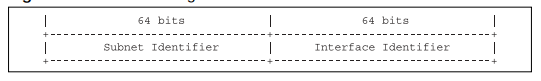
\includegraphics[width=0.71\textwidth]{v6vsv4.png}
 \caption[Comparaciones]{Comparación entre IPv4 e IPv6}
\end{figure} \par

Las direcciones MAC hoy en día solo son de 48-bits de longitud para 16 bits en el id de interfaz que 
es reservado. En contraste IPv4 son 32 bits de longitud.Estas también están comprendidas en un 
numero de subred. En IPv4 los administradores de red asignan tanto el numero de subred como el 
número de host.
\subsection{Administración de Direcciones}
IPv6 cuenta con un prefijo de subred de 64 bits, que se subdivide en cinco campos que se ilustrarán 
en la figura siguiente, el primer campo es el de prefijo de formato(fp) que identifica una 
unidifusión global agregable. El tercero se reserva para uso futuro
\begin{figure}[h!]
 \centering
 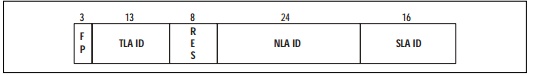
\includegraphics[width=0.71\textwidth]{asign.png}
 \caption[Asignación de prefijo]{Prefijo de subred de la dirección unicast}
\end{figure} \par
La clave para el entendimiento de IPv6 son dos campos: el TLA ID y el NLA ID. Apoyan a una 
direccionamiento jerárquico. Direcciones IPv6 globales se asignan a los proveedores de servicios o de 
organizaciones TLA, las organizaciones a su vez asignan espacio para la agregación del siguiente 
nivel NLA. Esta jerarquía que IPv4 no tiene estimula la agregación de direcciones para reducir el 
tamaño del núcleo de las tablas de enrutamiento. Por otra parte en IPv4 las direcciones son 
comúnmente asignadas por bloques CIDR. Cada bloque CIDR se compone de una o mas direcciones de clase 
C. Cada bloque de clase C puede tratar aproximadamente 254 dispositivos. Desafortunadamente los 
bloques CIDR tienen asignadas a diferentes organizaciones no pueden ser fácilmente agregados y cada 
bloque CIDR requiere una entrada en la tabla de enrutamiento separada de un router. El núcleo de 
estos bloques ha provocado un crecimiento explosivo en el tamaño del núcleo de la tablas de 
enrutamiento cosa que perjudica a la velocidad de enrutamiento ya que al ser mas grande la tabla, 
cuesta mas trabajo encontrar la dirección destino.\par
El administrador no deberá preocuparse por la configuración de la red como ya hemos mencionado.Las 
direcciones globales unicast no requieren traducción de direcciones cuando se utiliza para acceder a
redes externas tales como la Internet. En IPv4, los espacios de direcciones privadas se utilizan 
cuando las direcciones son globales, entonces deben traducirse a un conjunto limitado de direcciones 
globales cuando se accede a redes externas.

\begin{figure}[h!]
 \centering
 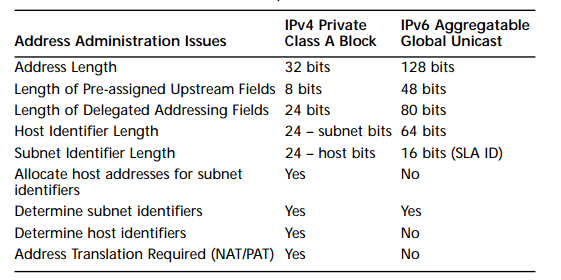
\includegraphics[width=0.71\textwidth]{aaip46.png}
 \caption[Comparativo IPv4, IPv6]{Comparativo de administración de direcciones IPv6 vs IPv4}
\end{figure} \par

\subsubsection{Comparación de cabeceras}
IPv6 ofrece una cabecera mas ágil que la de IPv4. Se eliminan cinco campos incluyendo el de longitud 
variable que existe en IPv4, los campos del primero cuentan con formato fijo de cuarenta bytes.

\begin{figure}[h!]
 \centering
 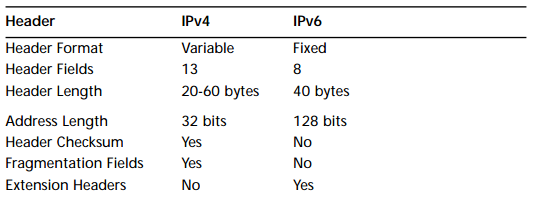
\includegraphics[width=0.71\textwidth]{compcab.png}
 \caption[Comparativo de cabeceras]{Comparativo de cabeceras }
\end{figure} \par

Sin embargo IPv6 cuenta con unos cabeceras adicionales que solo nombraremos, ya que los mas 
importantes fueron detallados en la sección anterior:
\begin{itemize}
\item Cabecera ``Salto a Salto" 
\item Cabecera de opción a destino
\item  Cabecera  de Ruteo
\item Cabecera de Fragmentación
\item Cabecera de Autenticación
\item  Cabecera ESP
\end{itemize}

\subsection{Conclusión de la Comparación}
Para ir finalizando la sección, presentaremos un cuadro comparativo que resumirá las comparaciones 
tratadas aquí.

\begin{figure}[h!]
 \centering
 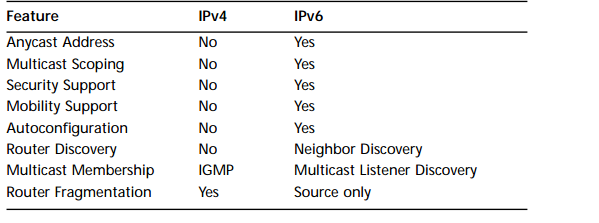
\includegraphics[width=0.71\textwidth]{comp.png}
 \caption[Diferencias]{Diferencias entre protocolos}
\end{figure} \par

IPv6 proporciona seguridad integrada compatible con el uso de cabeceras de autenticación y cifrado, 
para la movilidad proporciona funciones de agente interno y direcciones de atención.Ofrece un plug 
and play y la dirección del host puede ser configurada automáticamente. IPv4 no tiene incorporada la 
función de autoconfiguración, por lo tanto no puede configurar obteniendo parámetros de las fuentes 
externas tales como servidores DNS. IPv4 se basa en aumentaciones tales como 
\textbf{IGMP}\footnote{Internet Group Management Protocol} e IPv6 tiene 
\textbf{MLD}\footnote{Multicast Liner Discovery} que permite determinar cual de los puertos 
contienen oyentes de multidifusion.
IPv4 fragmenta paquetes para para poder transportar paquetes muy grandes, lo que satura la red, 
IPv6 solo permite el nodo de origen para fragmentar un paquete. Proporciona una ruta de MTU 
Discovery function que permite que la fuente del paquete fragmente los paquetes de forma eficiente. 
Esto elimina la necesidad de los dispositivos de red para fragmentar aun mas un paquete a lo largo 
de la transferencia.

\section{Implementar IPv6}
\subsection{Estado Actual}
La adopción de IPv6 no se a dado tan rápidamente como sus diseñadores lo esperaban. Dado que el 
estándar no es retro compatible con IPv4 ambos lados, tanto como clientes como servidores deben 
implementarlo para hacer uso de el y dado que no se provee un mayor beneficio que mayor cantidad de 
direcciones la recepción fue tibia. Sin embargo con el próximo fin de la disponibilidad de la 
version 4, cada vez mas redes empezaron a soportar IPv6.\par
A fines de la década pasada IPv6 a pesar de cumplir casi una década, presentaba una penetración en 
el mercado muy baja, un revelamiento de Google demostró en 2008 que el estándar representaba menos
del 1\%, aproximadamente 0.238\% del trafico de los países\cite{googleIPv6}.\par
Ya adentrándonos en nuestra actual década mas precisamente Octubre 2011 la capacidad para dar un 
servicio en IPv6 era sustancialmente mas alta llegando a un 85\% de los proveedores de internet del 
nivel superior y el soporte global había llegado a un 12\% del total. El soporte de software también 
se había masificado con los principales SO soportando IPv6. En ese 
mismo año para el mes de Junio y en el día 8 la \emph{Internet Society} organizo el \textbf{World 
IPv6 Day}. La cual fue una prueba mundial de un día de duración donde la grandes empresas 
desplegaron sus tecnologías IPv6, la prueba fue un éxito y vio aumentada el escaso trafico de la 
nueva version, también ayudo a mejorar los stacks duales, se implementa lado a lado IPv4 y v6. 
Incluso algunas como facebook decidieron dejar sus servicios v6.\par
Al año (2012) siguiente la misma sociedad organizo el \textbf{World IPv6 Launch Day}, con la 
diferencia que esta vez el despliegue debía ser permanente y no solo por un día. Todas estas medidas 
han logrado que el uso aumente actualmente llegando actualmente al 1.14\%. Actualmente Rumania, 
Francia, Alemania, Japon y EE.UU. son los países con mayor adopción del protocolo con Rumania 
llegando al 8.85\% el mas alto del mundo, en latinoamerica Peru se encuentra en la avanzada con un 
1.1\%.
\begin{figure}[h!]
 \centering
 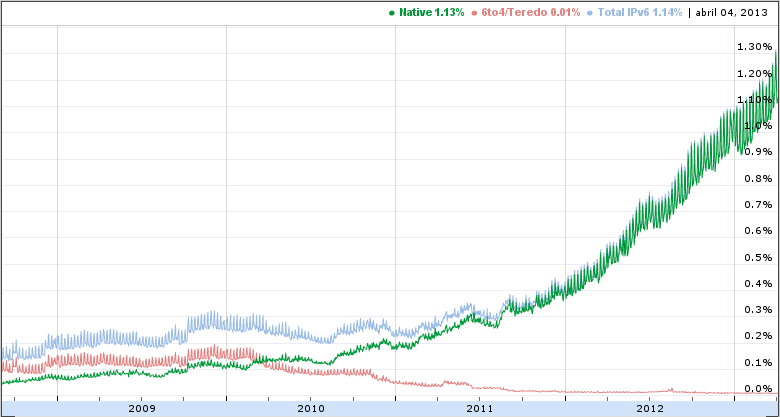
\includegraphics[width=0.79\textwidth]{adopcionIPv6.png}
 \caption[Adopción Global de IPv6]{Adopción Global de IPv6}
\end{figure}

\subsection{Mecanismos de Transición}
Dado que la penetración en el mercado es muy baja y ya se han agotado en ciertas regiones la 
direcciones existentes se debe de buscar una solución, pero el problema radica en la 
incompatibilidad de los protocolos, no se puede pasar a IPv6 y que este de servicio al estándar 
anterior y realizar un paso gradual. Tampoco es factible apagar todos los servidores y clientes IPv4 
y pasar a IPv6, asi que se debe de buscar una solución o soluciones de compromiso.\par
Una solución posible se encuentra disponible y se la llama dual-stack.
En este caso se necesita contar con suficiente cantidad de direcciones IPv4 para poder desplegar las 
dos versiones del protocolo en simultáneo en toda la red. De esta forma, cuando se establece una 
conexión hacia un destino sólo IPv4, se utilizará la conectividad IPv4 y si es hacia una dirección 
IPv6, se utilizará la red IPv6. En caso que el destino tenga ambos protocolos, normalmente se 
preferirá intentar conectar primero por IPv6 y en segunda instancia por IPv4.
\begin{figure}[h!]
 \centering
 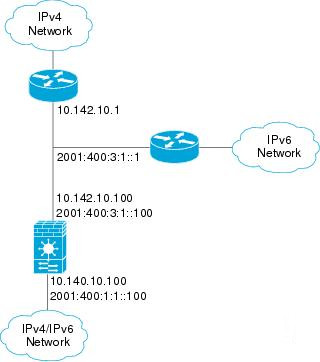
\includegraphics[width=0.4\textwidth]{dual_stack.jpg}
 \caption[Dual Stack]{Dual Stack}
\end{figure}\par
Otra solución en existencia no tan deseable como la anterior, pero sin lugar a dudas efectiva es el 
tunneling (Figura ~\ref{fig:IPv6_Tunneling}).
Es uno de los mecanismos mas antiguos para poder atravesar redes que no tienen soporte nativo del 
protocolo que se está utilizando. En general se utilizan túneles encapsulando IPv6 dentro de IPv4, 
permitiendo de esta forma atravesar redes que no manejan IPv6, pero también podemos encontrar la 
situación inversa. Los paquetes originales son transportados hasta un punto de la red por medio del 
protocolo original, luego encapsulados para atravesar la porción de red que no lo soporta y luego 
des-encapsulados en el otro extremo para ser enviados al destino final en forma nativa.
Los túneles mas habituales son los túneles manuales y los túneles automáticos. Los túneles manuales 
se deben configurar explícitamente en algún equipo de la red, mientras que los automáticos se 
configuran automáticamente en algunos sistemas operativos. En el caso de los primeros, podemos citar 
los túneles manuales entre dos equipos o mediante "tunnel brokers". En el segundo caso, los más 
conocidos son 6to4 y Teredo.
Dentro de los mecanismos de encapsulado podemos mencionar también la técnica conocida como 6PE/6VPE, 
que se utiliza para encapsular el tráfico IPv6 por parte de carriers que tienen redes MPLS.
\begin{figure}[h!]
 \centering
 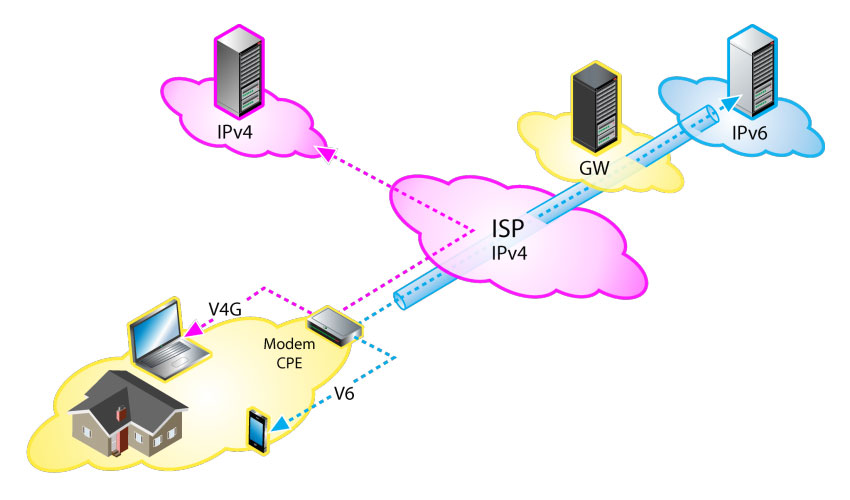
\includegraphics[width=0.57\textwidth]{ipv6_tunnel.jpg}
 \caption[IPv6 Tunneling]{IPv6 Tunneling}
 \label{fig:IPv6_Tunneling}
\end{figure}\par
Por ultimo analizaremos el método de traducción (Figura ~\ref{fig:IPv6_traduc}), esta técnica 
consiste en utilizar algún dispositivo en la red que convierta los paquetes de IPv4 a IPv6 y 
viceversa. Ese dispositivo tiene que ser capaz de realizar la traducción en los dos sentidos de 
forma de permitir la comunicación. Dentro de esta clasificación podemos mencionar NAT64/DNS64: la 
red es IPv6 nativa y para llegar a sitios que son sólo IPv4 se realiza una traducción al estilo NAT, 
mediante un mapeo entre los paquetes IPv6 e IPv4. Se utiliza un prefijo especial para mapear 
direcciones IPv4 a IPv6: 64:ff9b::/96. Es necesario también utilizar una modificación al DNS, 
llamada DNS64, que permite generar un registro AAAA aún cuando el destino no tenga dirección IPv6 
(es decir, el DNS responda sólo con registros de tipo A). Vale la pena mencionar que una de las 
propuestas iniciales de mecanismos de traducción fue NAT-PT (RFC 2766), que al dia de hoy ha sido 
desaconsejado debido a sus fallas (ver RFC 4966) y ha sido reclasificado como ``histórico" por la 
IETF.

\begin{figure}[h!]
 \centering
 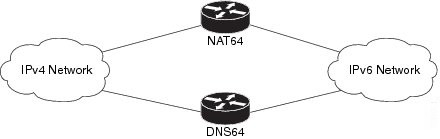
\includegraphics[width=0.57\textwidth]{ipv6_translation.jpg}
 \caption[Traducción IPv6]{Traducción IPv6}
 \label{fig:IPv6_traduc}
\end{figure}

\section{Conclusión}
Como se puede apreciar aunque el peligro del agotamiento de direcciones es real y hasta en ciertos 
lugares ya a sucedido, y la superioridad de IPv6 en otros aspectos no se a visto una gran 
penetración en el mercado mundial. Lo cual a nuestro parecer se debe no solo a impedimentos técnicos 
sino a la estructura muy descentralizada de internet. No existen órganos mundiales con capacidad de 
guiar con mano de hierro la dirección de esta, solo se pueden presentar opciones y esta por consenso 
los acepta o no. Así a sido toda su historia siempre evoluciono a los que necesitaba cuando lo 
necesitaba y de la manera mas económica, no solo en lo monetaria sino en todos los recursos.\par
Quizás se podría utilizar una analogía con un ser vivo o una especie que evoluciona de a poco de la 
manera menos traumática posible, donde los cambios son dados por el ambiente siempre cambiante. 
Quienes implementan de mejor manera los cambios tienen la capacidad de seguir mas en el mercado y 
que perduren sus practicas o tecnologías, tal como lo hace la selección natural. De esta manera 
siempre se busca que los cambios sean para mejor y nadie puede imponer su agenda o intereses. Esto
ultimo se logra también por la gran cantidad de ``jugadores" presentes.\par
Pero tal solución no viene sin sus riesgos la característica de ser descentralizada le lleva a pasar
por estos problemas donde un cambio debe ser inmediato y global. Una situación que se torna muy 
difícil, el estado actual dice que IPv4 funciona bien por ahora sus deficiencias pueden ser 
mitigadas por otras tecnologías y el riesgo del cambio es bajo. Pero su mayor debilidad no puede ser 
arreglada con parches o tecnologías extras, se debe cambiar de raíz, un cambio que cualquier 
organismo aborrecería, por ser muy extremo y costoso.\par
Igual el futuro no se presenta oscuro ni mucho menos y si lo que la historia nos demuestra es que el 
negocio, definido por la totalidad de la internet, siempre adopta los cambios que le permiten crecer 
mas. Aunque IPv6 avance mas lento de lo esperado, sus beneficios son muy grandes para ser dejados de 
lado en pos de la seguridad de IPv4. A fin de cuentas los organismos que se mantienen estáticos que
no evolucionan, se mueren. Internet aunque haya ocupado poco tiempo en nuestra historia se ha 
vuelto muy importante quizás una de esas tecnologías que permitieron a nuestra especie dar un salto 
cuántico, como la agricultura y la imprenta. IPv4 vivió mas tiempo del esperado y cumplió bien con 
su cometido pero ya es tiempo para que sea jubilado, ya demuestra sus años en contra de IPv6 y 
creemos firmemente que mercado, internet o como se lo quiera llamar lo dejara de lado de la mejor 
manera posible y ofrecerá el mejor servicio posible y a su vez enfocara su esfuerzo en otros 
inconvenientes por venir.

\newpage
\begin{thebibliography}{9}

\bibitem{redesTenem}
  Andrew S. Tanenbaum
  \emph{Redes de Computadoras}.
  USA,
  2003.

\bibitem{TaoIETF}
  Paul Hoffman
  \emph{The Tao of IETF: A Novice's Guide to the Internet Engineering Task Force}.
  USA,
  2012.
		
\bibitem{historyTCPiP}
  Gary C. Kessler
  \emph{An Overview of TCP/IP Protocols and the Internet}.
  USA,
  9 Nov 2010.
		
\bibitem{poolIPv4}
 nro.net
 \emph{Free Pool of IPv4 Address Space Depleted.} 
 19 Mar 2013\\
	\url{https://www.nro.net/news/ipv4-free-pool-depleted}	

\bibitem{IPv6 Architecture}
 cu.ipv6ft.org 
 \emph{Introduction to IPv6 Architecture.} 
 26 Mar 2013\\
	\url{http://www.cu.ipv6tf.org/literatura/sample.pdf}

\bibitem{googleIPv6}
 Steinar H. Gunderson
 \emph{Global IPv6 Stadistics}
 Nov 2008\\
 \url{http://meetings.ripe.net/ripe-57/presentations/Colitti-Global_IPv6_statistics_-
 _Measuring_the_current_state_of_IPv6_for_ordinary_users_.7gzD.pdf}
		
\bibitem{IPV6}
 ipv6.com\\
 \url{http://www.ipv6.com/}		
					
\end{thebibliography}

\end{document}
